\documentclass[a4paper,14pt]{article}

\usepackage{comment} % Para comentar várias linhas ao mesmo tempo

%matemática
\usepackage{amsmath}
\usepackage{amssymb}

%diagramação
\usepackage{extsizes}
\everymath{\displaystyle}
\usepackage{geometry}
\usepackage{fancyhdr}
\usepackage{multicol}
\usepackage{graphicx}
\usepackage[brazil]{babel}
\usepackage[shortlabels]{enumitem}
\usepackage{cancel}
\usepackage{textcomp}
\usepackage{tcolorbox}

%tabelas
\usepackage{array} % Para melhor formatação de tabelas
\usepackage{longtable}
\usepackage{booktabs}  % Para linhas horizontais mais bonitas
\usepackage{float}   % Para usar o modificador [H]
\usepackage{caption} % Para usar legendas em tabelas
\usepackage{wrapfig} % Para usar tabelas e figuras flutuantes

\begin{comment}
%tikzpicture
\usepackage{tikz}
\usepackage{scalerel}
\usepackage{pict2e}
\usepackage{tkz-euclide}
\usetikzlibrary{calc}
\usetikzlibrary{patterns,arrows.meta}
\usetikzlibrary{shadows}
\usetikzlibrary{external}
\end{comment}
	
%pgfplots
\usepackage{pgfplots}
\pgfplotsset{compat=newest}
\usepgfplotslibrary{statistics}
\usepgfplotslibrary{fillbetween}

%colours
\usepackage{xcolor}



\columnsep=2cm
\hoffset=0cm
\textwidth=8cm
\setlength{\columnseprule}{.1pt}
\setlength{\columnsep}{2cm}
\renewcommand{\headrulewidth}{0pt}
\geometry{top=1in, bottom=1in, left=0.7in, right=0.5in}

\pagestyle{fancy}
\fancyhf{}
\fancyfoot[C]{\thepage}

\begin{document}
	
	\noindent\textbf{6FMA77 - Matemática} 
	
	\begin{center}Divisão de decimais (II) (Versão estudante)
	\end{center}
	
	\noindent\textbf{Nome:} \underline{\hspace{10cm}}
	\noindent\textbf{Data:} \underline{\hspace{4cm}}
	
	%\section*{Questões de Matemática}
	
	\begin{multicols}{2}
		\noindent Para dividirmos dois números decimais, igualamos o número de casas decimais, "cortamos" a vírgula e, em seguida, usamos o algoritmo da divisão que já conhecemos. \\
		Exemplo: \\
		0,108 : 1,2 \\
		\begin{center}
		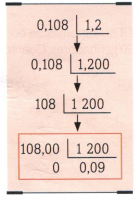
\includegraphics[width=0.7\linewidth]{6FMA77_imagens/imagem1}
		\end{center}
		\noindent\textsubscript{-----------------------------------------------------------------------}
    	\begin{enumerate}
   			\item Calcule.
   			\begin{enumerate}[a)]
   				\item 2,8 : 0,4  \\\\\\\\\\\\\\\\
   				\item 20,25 : 2,25 \\\\\\\\\\\\
   				\item 8,5 : 0,04 \\\\\\\\\\\\
   				\item 0,1296 : 21,6 \\\\\\\\\\\\
   			\end{enumerate}
   			\item Júlio está fazendo uma rabiola para sua pipa. Ele colocará uma tira de plástico no começo da rabiola e a cada 0,15 m de linha ele colocará outra tira. De quantas tiras ele precisará para fazer 3,24 m de rabiola? \\\\\\\\\\\\
   			\item Na festa de seu filho, Joana distribuiu refrigerante para as crianças. Cada uma tomou 750 mL, totalizando 12 garrafas de 1,5 L cada. Sabendo-se que 1mL = 0,001 L, quantas crianças havia na festa? \\\\\\\\\\\\\\\\\\\\
   			%16 a 19
   			\item Calcule.
   			\begin{enumerate}[a)]
   				\item 3,7 : 0,4 \\\\\\\\
   				\item 8,32 : 0,64 \\\\\\\\
   				\item 0,54 : 0,8 \\\\\\\\
   				\item 8,364 : 0,06 \\\\\\\\
   				\item 1,3 : 0,06 \\\\\\\\
   				\item 0,007 : 0,3 \\\\\\\\
   				\item 8 : 0,00032 \\\\\\\\
   				\item 7 : 1,75 \\\\\\\\
   			\end{enumerate}
   			\item Daniela pretende fazer pulseiras e, para cada uma, ela utiliza 0,16 m de fio. Se ela comprar um fio de 3,2 m de comprimento, quantas pulseiras Daniela poderá fazer? \\\\\\\\\\\\\\\\\\\\\\\\\\
   			\item Explique por que, ao dividirmos um número positivo por 0,2, obtemos um quociente maior que o divisor \\\\\\\\\\\\\\\\\\\\\\\\\\\\\\\\\\\\\\\\\\\\\\\\\\\\\\\\\\\\\\\\\\\\\\\\\\
   			\item Por que devemos igualar o número de casas à direita da vírgula de dois decimais e, em seguida, tirar as vírgulas quando dividimos um pelo outro? (Dica: escreva a divisão como fração.) \\\\\\\\\\\\
   		\end{enumerate}
        $~$ \\ $~$ \\ $~$ \\ $~$ \\ $~$ \\ $~$ \\ $~$ \\ $~$ \\ $~$ \\ $~$ \\ $~$ \\ $~$ \\ $~$ \\ $~$ \\ $~$ \\ $~$ \\ $~$ \\ $~$ \\ $~$ \\ $~$ \\ $~$ \\ $~$ \\ $~$ \\ $~$ \\ $~$ \\ $~$ \\ $~$ \\ $~$ \\ $~$
        \end{multicols}
\end{document}